% =========================================================================
% REMIX v5 — sections/experiments.tex
% Composition: v4 full replacement (5.1–5.3) + v5 controlled study (5.4,
% moved before the leverage section) + v5 "When can pooling pay?" (5.5).
% All REMIX rows and margins use the audited configurations.
% =========================================================================

% =========================================================================
\section{Experiments}\label{sec:experiments}
% =========================================================================

\subsection{Experimental design}\label{sec:setup}

\textbf{Datasets.} We evaluate on two daily panels---\textbf{Online
Retail} \citep{chen2015} (3{,}649 series) and a seed-controlled
5{,}000-series \textbf{M5} sample \citep{makridakis2022}---and the
monthly intermittent suite of \citet{damato2025}: \textbf{Auto}
(3{,}000 series), \textbf{Carparts} (2{,}509), and \textbf{RAF}
(5{,}000). Together they contain more than 19{,}000 series and span
long daily histories and short, highly sparse monthly panels. Dataset
construction and holdout lengths are in Appendix~\ref{app:datasets}.
Both the probabilistic and the point M5 protocols use the first two
thirds of each series for initialization.

\textbf{Comparators.} The classical set comprises Croston, SBA, TSB,
ADIDA, and IMAPA; stronger statistical comparators are AutoARIMA,
AutoTheta, a per-series autoregressive Tweedie GLM, iETS, and the official
TweedieGP implementation on the three monthly panels. For probabilistic
evaluation we use native distributions where available and chronological
split-conformal wrappers (CP-$\ast$) for the point forecasters. The
Online Retail walk-forward study additionally includes adaptive conformal
inference (ACI) applied to ADIDA and TSB. A 25-candidate tuned-TSB control
receives the same internal chronological selection budget as \REMIX{}.
DeepState and Chronos-Bolt comparisons are confined to
Appendix~\ref{app:neural} because they use subset or proxy protocols.
Implementation details and complete settings are in
Appendix~\ref{app:implementation}.

\textbf{Protocols and metrics.} The primary fixed-origin experiment fits
once on the initialization window and scores the full evaluation span.
A strict walk-forward experiment then reveals and updates one block at a
time: seven-day blocks on Online Retail and one-month blocks on Carparts.
Classical and conformal methods refit each block except Online Retail
AutoARIMA, AutoTheta, and iETS, which refit every four blocks; \REMIX{}
updates discounted sufficient statistics each block. The primary metric is
scaled pinball loss (SPL; lower is better), averaged over
$q\in\{0.1,0.25,0.5,0.75,0.9\}$; we separately report q90 and the far tail
because inventory decisions are asymmetric. All quantiles are
zero-truncated and monotonized, and \REMIX{} is reported without post-hoc
calibration. Every model in Table~\ref{tab:prob} is scored by one
implementation from its stored quantile predictions, so no cell mixes
scoring versions. Fixed-origin, walk-forward, and subset foundation model
results are kept separate because they answer different questions. MAE and
RMSSE are secondary diagnostics rather than the headline criteria because
zero forecasts can minimize absolute error on intermittent panels. Full
point, interval, significance, and efficiency results are in
Appendix~\ref{app:extra}.

% =========================================================================
\subsection{Probabilistic forecasting across panels}
\label{sec:main-results}
% =========================================================================

\begin{table*}[t]
\centering
\caption{\textbf{Probabilistic forecasting is the primary comparison.}
Scaled pinball loss (SPL; lower is better) is reported as the mean over
$q\in\{0.1,0.25,0.5,0.75,0.9\}$ and at q90. Bold and underline mark the
best and second-best non-degenerate methods. M5 reports seed 42 for direct
comparability; three-seed robustness is summarized in the text. \REMIX{}
uses its raw predictive law, with no post-hoc calibration. TweedieGP is the
official implementation and is evaluated on the three monthly panels for
which the authors released it. The all-zero row is a metric diagnostic and
is excluded from ranking.}
\label{tab:prob}
\small
\setlength{\tabcolsep}{3.2pt}
\begin{tabular}{lcc@{\hspace{9pt}}cc@{\hspace{9pt}}cc@{\hspace{9pt}}cc@{\hspace{9pt}}cc}
\toprule
 & \multicolumn{2}{c}{Online Retail} & \multicolumn{2}{c}{M5} & \multicolumn{2}{c}{Auto} & \multicolumn{2}{c}{Carparts} & \multicolumn{2}{c}{RAF}\\
\cmidrule(lr){2-3}\cmidrule(lr){4-5}\cmidrule(lr){6-7}\cmidrule(lr){8-9}\cmidrule(lr){10-11}
Model & Mean & q90 & Mean & q90 & Mean & q90 & Mean & q90 & Mean & q90\\
\midrule
AutoARIMA & 1.0069 & 1.6297 & 1.7919 & 2.4148 & 0.3189 & 0.2659 & 0.4084 & 0.4897 & 0.4020 & 0.5910\\
AutoTheta & 1.0055 & \secondbest{1.6056} & 1.7954 & 2.3123 & 0.3403 & 0.2760 & 0.3925 & \secondbest{0.4697} & 0.4104 & 0.5956\\
CP-Croston & 1.5502 & 2.7686 & \secondbest{1.6902} & \best{2.1551} & 0.3260 & 0.3105 & 0.4012 & 0.5433 & 0.3322 & 0.4927\\
CP-SBA & 1.5492 & 2.8601 & 1.6939 & \secondbest{2.1736} & 0.3256 & 0.3153 & 0.3982 & 0.5418 & 0.3290 & 0.4920\\
CP-TSB & 1.1744 & 2.6746 & 1.8794 & 2.3148 & 0.3459 & 0.3150 & 0.3783 & 0.4842 & 0.3814 & 0.4986\\
CP-ADIDA & 1.1239 & 2.5409 & 1.7150 & 2.1949 & 0.3275 & 0.3082 & 0.3571 & 0.4982 & 0.3097 & 0.4905\\
CP-IMAPA & 1.1280 & 2.5506 & 1.7190 & 2.1904 & 0.3279 & 0.3084 & 0.3561 & 0.4908 & 0.3116 & 0.4907\\
Tweedie-GLM & 1.1477 & 1.7458 & 4.0693 & 5.2620 & 0.3221 & 0.2783 & 0.4776 & 0.6897 & 0.3121 & 0.5312\\
iETS & \secondbest{0.9846} & 1.7544 & 2.0282 & 2.9772 & 0.3448 & 0.3252 & 0.4561 & 0.5646 & 0.3494 & \secondbest{0.4900}\\
TweedieGP & --- & --- & --- & --- & \secondbest{0.2985} & \best{0.2598} & \best{0.3214} & \best{0.4600} & \secondbest{0.2763} & 0.5219\\
\midrule
Zero (diagnostic) & 0.9161 & 1.6490 & 1.9590 & 3.5262 & 0.5612 & 1.0102 & 0.3736 & 0.6725 & 0.2669 & 0.4805\\
\midrule
\REMIX{} (ours) & \best{0.8849} & \best{1.5268} & \best{1.6707} & 2.4758 & \best{0.2937} & \secondbest{0.2599} & \secondbest{0.3229} & 0.4817 & \best{0.2680} & \best{0.4856}\\
\bottomrule
\end{tabular}
\end{table*}

Table~\ref{tab:prob} sets the empirical position, and it is a narrow one.
\REMIX{} attains the lowest mean SPL on four of the five panels; the
official TweedieGP implementation wins Carparts ($0.3214$ versus
$0.3229$). The margins over the strongest comparator vary by an order of
magnitude across panels: $10.1\%$ on Online Retail, $3.0\%$ on RAF,
$1.6\%$ on Auto, and $1.2\%$ on M5. Across three independent
5{,}000-series M5 samples the selected configuration is identical---%
$(\text{mixture},\,w{=}0.95,\,K{=}6)$---and \REMIX{} has mean SPL
$1.7501\pm0.084$ against $1.7547\pm0.065$ for CP-Croston, its closest
comparator: ahead on two samples, behind by $1.0\%$ on the third, and
ahead on average by $0.3\%$, well within one standard deviation. We report
the spread rather than an aggregate win because it is the quantity
Section~\ref{sec:leverage} explains. The explanation is not that these
panels leave no room for a hierarchical construction to work; on three of
them the credibility weights say otherwise. It is that the room which
exists is not converted by a learned partition, which is why the
achievable margin is set by the shared predictive law rather than by the
pooling structure.

The degenerate row exposes what the central quantiles cannot see. On RAF,
the all-zero forecast is marginally better through q90 because the true
quantiles of most series are zero. At $q\in\{0.95,0.975,0.99\}$ it falls
behind every intensity-bearing method, and intensity-bearing models become
distinguishable from one another (Appendix~\ref{app:fartail}). TweedieGP
is strongest throughout the Carparts far tail and remains competitive on
RAF. The probabilistic claim is therefore not that one distribution wins
every quantile, but that \REMIX{} is the most consistent aggregate
performer across panels and remains informative in the region where a zero
forecast ceases to be useful.

Point forecasts tell a deliberately weaker story. \REMIX{} is best on six
of ten MAE/RMSSE cells and top two on seven, but the zero forecast has the
lowest MAE on three panels and classical methods lead several remaining
cells. We report the complete point table and horizon decomposition in
Appendix~\ref{app:point}: they establish competitiveness and rule out a
long-horizon averaging artifact, but do not support uniform point-forecast
superiority.

% =========================================================================
\subsection{Strict walk-forward forecasting}\label{sec:walkforward}
% =========================================================================

\begin{table*}[t]
\centering
\caption{\textbf{Strict probabilistic walk-forward evaluation.}
Online Retail uses seven-day blocks and Carparts uses monthly blocks.
Mean and q90 are scaled pinball losses; Cov.$^{+}$ is 80\% interval
coverage conditional on positive demand and AIW is average interval
width. Dashes denote an unevaluated panel. AutoTheta refits every four
Online Retail blocks; the classical wrappers, ACI, and all Carparts
baselines refit each block. \REMIX{} updates sufficient statistics each
block. Bold and underline rank non-degenerate methods by SPL.}
\label{tab:wfprob}
\footnotesize
\setlength{\tabcolsep}{4.0pt}
\begin{tabular}{lrrrrrrrr}
\toprule
 & \multicolumn{4}{c}{Online Retail} & \multicolumn{4}{c}{Carparts}\\
\cmidrule(lr){2-5}\cmidrule(lr){6-9}
Model & Mean & q90 & Cov.$^{+}$ & AIW & Mean & q90 & Cov.$^{+}$ & AIW\\
\midrule
AutoTheta & 1.0586 & \secondbest{1.4835} & 0.765 & 16.43 & 0.4056 & \secondbest{0.4743} & 0.678 & 1.80\\
CP-TSB & 1.3733 & 2.8422 & 0.468 & 5.71 & 0.3836 & 0.4758 & 0.551 & 1.27\\
CP-ADIDA & 1.1576 & 2.5143 & 0.473 & 5.47 & 0.3509 & 0.4880 & 0.593 & 1.28\\
CP-IMAPA & 1.1773 & 2.5224 & 0.471 & 5.47 & \secondbest{0.3492} & 0.4789 & 0.581 & 1.27\\
ACI-ADIDA & \secondbest{0.9108} & 1.6681 & 0.646 & 19.67 & --- & --- & --- & ---\\
Zero (diagnostic) & 0.9161 & 1.6490 & 0.000 & 0.00 & 0.3736 & 0.6725 & 0.000 & 0.00\\
\midrule
\REMIX{} & \best{0.8540} & \best{1.4002} & 0.621 & 10.31 & \best{0.3145} & \best{0.4578} & 0.669 & 1.41\\
\bottomrule
\end{tabular}
\end{table*}

Table~\ref{tab:wfprob} is the deployment-facing test. On Online Retail
\REMIX{} improves mean SPL by $6.2\%$ over ACI-ADIDA and q90 by $5.6\%$
over AutoTheta, the strongest q90 comparator. On Carparts it improves mean
SPL by $9.9\%$ over CP-IMAPA and wins all five quantiles.

Three features of this table deserve more attention than the margins.
First, \emph{the choice of conformal construction matters more here than
the choice of forecaster}: making the wrapper adaptive
\citep{gibbs2021} improves ADIDA's mean SPL from $1.1576$ to $0.9108$, a
$21\%$ gain that is more than three times the remaining gap to \REMIX{}.
Static split-conformal wrappers are the standard probabilistic baseline in
this literature; on this evidence they understate what conformal
prediction can do on intermittent panels, and comparisons drawn against
them---including earlier versions of our own---are correspondingly
generous. Second, \emph{coverage and sharpness separate}. ACI-ADIDA
attains higher positive-demand coverage ($0.646$ versus $0.621$) with
intervals almost twice as wide ($19.67$ versus $10.31$); neither method
dominates, and the SPL ordering reflects sharpness rather than
calibration. Third, \emph{the central quantiles carry little information
on the sparse panel}: on Carparts the q10 and q25 entries of \REMIX{}
equal the all-zero forecast exactly and q50 sits marginally below it, so
essentially the entire mean-SPL difference is generated above the median.
We return to this in Appendix~\ref{app:fartail}, where the far-tail
levels are the only ones that separate intensity-bearing models on the
sparsest panels.

The configuration is selected once at the origin and then updated online;
repeated online re-selection is outside the present experiment.

% =========================================================================
\subsection{Controlled test of the resolution mechanism}
\label{sec:synthetic}
% =========================================================================

Real data never reveal the true pooling partition, so on their own they
cannot distinguish a partition that is not worth having from one we failed
to find. Both appear as a small number. We therefore construct panels
where the partition is correct by definition, and use them as a reference
against which the learned partitions of Section~\ref{sec:leverage} are
measured: what a good partition is worth at a given level of credibility
leverage, rather than what our estimator obtains there.

We simulate from the hierarchical hurdle model of \eqref{eq:model} with
group centers arranged symmetrically around a fixed grand mean, so that
increasing separation does not change the panel scale. Each cell compares
a single pool against the known true partition under the same predictive
representation, with nine paired replicates, and sweeps the two quantities
that Section~\ref{sec:resolution} identifies as controlling credibility:
the discount $w$ and the series length $T$. The resulting grid spans the
leverage range the real panels occupy, from the near-fully-shrunk regime
of Carparts to the item-dominated regime of Auto and RAF.

\begin{table}[t]
\centering
\caption{Advantage of the \emph{true} partition over a single pool on
simulated panels (mean percentage improvement over nine paired replicates;
standard error in parentheses). Positive favors the partition. $T$ is
series length.}
\label{tab:sanity}
\small
\setlength{\tabcolsep}{3.5pt}
\begin{tabular}{llrrrr}
\toprule
$T$ & $w$ & NLL & log-size MSE & pinball & MAE\\
\midrule
$30$ & $0.90$ & $2.40\;(0.18)$ & $17.15\;(2.39)$ & $2.25\;(0.61)$ & $-1.72\;(0.73)$\\
$30$ & $0.95$ & $1.12\;(0.39)$ & $9.00\;(2.45)$ & $-0.44\;(0.58)$ & $-0.17\;(0.51)$\\
$30$ & $1.00$ & $1.02\;(0.08)$ & $8.37\;(1.53)$ & $-0.69\;(0.32)$ & $-1.95\;(0.59)$\\
$120$ & $0.90$ & $1.65\;(0.22)$ & $18.36\;(1.56)$ & $1.57\;(0.64)$ & $-3.34\;(1.37)$\\
$120$ & $0.95$ & $0.96\;(0.11)$ & $3.65\;(0.77)$ & $0.23\;(0.28)$ & $-1.32\;(0.73)$\\
$120$ & $1.00$ & $0.23\;(0.04)$ & $1.13\;(0.31)$ & $-0.32\;(0.13)$ & $-0.80\;(0.11)$\\
\bottomrule
\end{tabular}
\end{table}

Table~\ref{tab:sanity} gives the result. The true partition improves NLL
and log-size MSE in every cell, and pinball loss whenever forgetting is
strong; in a separate length sweep its pinball advantage decays from
$1.53\%$ at $T=12$ to $0.01\%$ at $T=400$. Both patterns follow the
credibility mechanism directly. Discounting or short histories reduce an
item's own weight $\lambda^{(+)}_i$ and open room for a prior to act;
long undiscounted histories drive $\lambda^{(+)}_i\to1$ and make every
partition irrelevant. Stronger forgetting simultaneously makes group
variance components harder to estimate, as
Proposition~\ref{prop:twosided} predicts, which is why the gains in the
$w=0.90$ rows are bought against a noisier $\hat\tau_g^2$ and do not
continue to grow without limit.

MAE moves the other way in all six cells. A known-correct partition, on
data generated from the model it describes, is reported as harmful by the
metric most commonly used in this literature. We take this as the cleanest
available statement of why Section~\ref{sec:main-results} treats
absolute-error criteria as diagnostics rather than as the headline.

\paragraph{What these panels are for.}
Plotted against median $\lambda^{(+)}$, the cells of
Table~\ref{tab:sanity} and the length sweep trace the grey curves of
Figure~\ref{fig:refinement-leverage}: the return to \emph{correct}
structure as a function of leverage. Because the partition is supplied
rather than estimated, that return is an upper envelope---no procedure
that must also learn the grouping can exceed it, and any procedure that
falls below it is losing something to estimation rather than to a lack of
structure. This is the comparison Section~\ref{sec:leverage} draws, and it
is the reason the controlled study is necessary rather than decorative:
the real panels supply the leverage coordinates, and only a known-partition
experiment can supply the ordinate they should be judged against.

Two boundaries apply. The experiment isolates the value of correct
structure and says nothing about whether the mixture recovers it---indeed
Section~\ref{sec:leverage} shows it does not, and the gap between the two
is precisely what the comparison measures. And it simulates from the model
that \REMIX{} fits, so the mechanism is tested under correct specification
only; a misspecified size law would shift the envelope, though it is hard
to see how it would raise it. Full diagnostics, including the growth of
$\mathrm{RMSE}(\hat\tau_g^2)$ as $w$ falls, are in
Appendix~\ref{app:simulation-details}.

% =========================================================================
\subsection{When can pooling pay?}\label{sec:leverage}
% =========================================================================

The results so far are consistent and small. This section asks whether
their size is a property of the data or of our estimator, and shows that
the two can be told apart with quantities the selector already computes on
the fitting head (Section~\ref{sec:select}).

\paragraph{What gets selected, and how weakly.}
All five panels select $w<1$: Carparts $0.90$, Online Retail and M5
$0.95$, Auto $0.99$, and RAF $0.997$. Across three independent
5{,}000-series M5 samples the selected configuration is identical in
structure, discount, and mixture order---$(\text{mixture},\,w{=}0.95,\,
K{=}6)$ in every case.

The pooling axis behaves differently, and the honest summary is that it
barely resolves. On three panels the spread between the best and worst
pooling structure at the selected discount is under a tenth of a percent
of validation SPL: $0.05\%$ on Online Retail, $0.08\%$ on Carparts,
$0.02\%$ on RAF. Only two panels separate at all---M5, where the learned
mixture beats the global pool by $0.58\%$, and Auto, where the global pool
beats every refinement by $0.31\%$. Announcing a winner on the other three
would report selector noise. What the selector reliably does is choose a
discount and avoid poor structural corners; it does not discover demand
taxonomies, and we do not claim it does.

\begin{table}[t]
\centering
\caption{\textbf{Credibility leverage under a single pool.} Median
credibility weight per panel at no forgetting and at the selected
discount, for both blocks of the hurdle model:
$\lambda^{(o)}_i=n_i/(n_i+\phi_g)$ for occurrence and
$\lambda^{(+)}_i=n_i^{+}/(n_i^{+}+\kappa_g)$ for positive size, the
latter being the quantity bounded by Proposition~\ref{prop:twosided}.
A weight near one means the item's own history dominates its posterior,
bounding how far any shared prior can move it. ``$<0.1$'' is the share of
items whose size-block weight falls below $0.1$. The final column is the
external MAE change of a separately selected learned partition relative to
the single pool; negative favors the single pool.}
\label{tab:leverage}
\small
\setlength{\tabcolsep}{3.0pt}
\begin{tabular}{lccccccc}
\toprule
 & & \multicolumn{3}{c}{$\lambda^{(+)}$ (size)} & \multicolumn{2}{c}{$\lambda^{(o)}$ (occ.)} & learned\\
\cmidrule(lr){3-5}\cmidrule(lr){6-7}
Panel & $w^{*}$ & $w{=}1$ & $w^{*}$ & $<0.1$ & $w{=}1$ & $w^{*}$ & vs.\ pool\\
\midrule
Carparts & $0.90$ & 0.802 & \textbf{0.224} & 22.5\% & 0.882 & 0.628 & $-1.2\%$\\
Online Retail & $0.95$ & 0.897 & \textbf{0.553} & 14.6\% & 0.969 & 0.895 & $-2.9\%$\\
M5 & $0.95$ & 0.996 & 0.841 & 12.9\% & 0.998 & 0.931 & $-2.3\%$\\
Auto & $0.99$ & 0.944 & 0.940 & 0.0\% & 0.525 & \textbf{0.422} & $-3.6\%$\\
RAF & $0.997$ & 0.926 & 0.917 & 0.0\% & 0.085 & \textbf{0.106} & $-31.5\%$\\
\bottomrule
\end{tabular}
\end{table}

\paragraph{Leverage is an upper bound, not a prediction.}
Table~\ref{tab:leverage} reports the diagnostic. Read as
Corollary~\ref{cor:resolution} intends, it does not say which partition
wins; it says how much any partition could win by. Two panels have almost
no room on the size block: Auto and RAF retain median
$\lambda^{(+)}\approx0.92$--$0.94$ even at their selected discounts, with
no item below $0.1$, so their sub-percent pooling differences are
explained before any partition is fitted. The remaining three do have
room. Carparts is extreme---median $0.224$, with $22.5\%$ of items
essentially fully shrunk---and Online Retail, at $0.553$ under the
selected discount, sits squarely in the regime where
Section~\ref{sec:synthetic} shows a supplied true partition earning more
than two percent.

\begin{figure}[t]
\centering
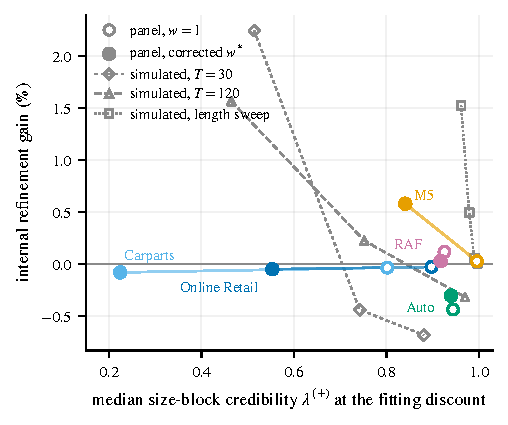
\includegraphics[width=\columnwidth]{figs/fig10a_refinement_leverage_size.pdf}\\[0.5em]
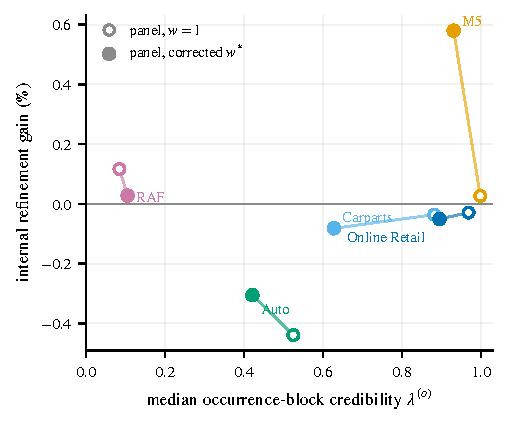
\includegraphics[width=\columnwidth]{figs/fig10b_refinement_leverage_occ.pdf}
\caption{\textbf{The simulated curves are an upper envelope that the real
panels do not reach.} Internal refinement gain (best refined structure
versus the global pool, validation SPL) against median credibility weight,
on the size block (top) and the occurrence block (bottom). Open markers
are $w{=}1$, filled markers the selected discount, and the connecting
segment is the movement forgetting induces. Grey curves are the controlled
panels of Section~\ref{sec:synthetic}, where the partition supplied is
correct by construction. Every real panel lies far below the envelope at
its own leverage---most visibly Online Retail, which the selected
discount moves into the high-return region of the size block while its
learned structure returns $-0.05\%$.}
\label{fig:refinement-leverage}
\end{figure}

\paragraph{What binds is learnability, not leverage.}
Figure~\ref{fig:refinement-leverage} places the real panels and the
controlled panels on the same axes, and the gap between them is the
section's main result. Where the partition is correct by construction, the
gain rises as leverage rises, reaching $+2.2\%$ near
$\lambda^{(+)}\approx0.5$. Where the partition must be learned, the gain
is between $-0.31\%$ and $+0.03\%$ on four panels and $+0.58\%$ on the
fifth, regardless of leverage. Online Retail is the decisive case: the
selected discount moves it to $\lambda^{(+)}=0.553$, inside the region
where the controlled study says a good partition is worth more than two
percent, and the mixture returns $-0.05\%$. The occurrence block behaves
the same way (Figure~\ref{fig:refinement-leverage}, bottom): RAF and Auto
occupy the low-$\lambda^{(o)}$ end, where the shared prior supplies most
of $\hat\pi_i$, and their refinement gains are still zero or negative.

This separates two explanations that aggregate results cannot. It is not
that these panels lack exploitable cross-series structure---the
credibility weights say the structure would be worth something if it were
correct. It is that the mixture objective does not recover a partition
worth shrinking toward. The binding constraint is learnability, and
Corollary~\ref{cor:resolution} bounds the prize rather than the shortfall.

\paragraph{High leverage is an amplifier with no sign attached.}
The clearest illustration is RAF, which combines the highest size-block
leverage in the panel set ($\lambda^{(+)}=0.917$) with the lowest
occurrence leverage ($\lambda^{(o)}=0.106$), and loses $31.5\%$ of
external MAE to a learned partition. The two facts are one fact. The point
forecast is $\hat y_i=\hat\pi_i\exp(\hat\mu_i+\hat\sigma_i^2/2)$; when
$89\%$ of $\hat\pi_i$ comes from the group prior, replacing the group is
close to replacing the forecast. This is the empirical content of the
caveat attached to Proposition~\ref{prop:active}: persistent prior leverage
guarantees that the choice of target keeps mattering, not that a
particular target is good. Read together with the previous paragraph, low
leverage caps the upside and high leverage uncaps the downside, and
neither makes a learned partition worth using here.

\paragraph{Forgetting is an order of magnitude larger.}
Computed within a single selection surface under one definition---the
M5 surface at its selected discount---refining the pooling
structure is worth $+0.58\%$ of validation SPL, while discounting at the
same structure is worth $8.95\%$ for the global pool and $9.46\%$ for the
mixture. The asymmetry that motivates the paper survives at an order of
magnitude, and it survives on the one panel where refinement is
measurable at all.

\begin{table}[t]
\centering
\caption{Online Retail distributional ablation. Each row is an
independent hierarchical run; ``auto'' denotes its own internal discount
selection. The raw predictive law is used and lower is better. Full
point metrics are in Appendix Table~\ref{tab:ablation-full}.}
\label{tab:ablation}
\small
\begin{tabular*}{\columnwidth}{@{\extracolsep{\fill}}llrrr@{}}
\toprule
Pooling & Forget & SPL & SPL$_{90}$ & AIW\\
\midrule
global & off & 0.8899 & 1.5306 & 10.51\\
taxonomy & off & 0.8897 & 1.5299 & 10.56\\
learned & off & 0.8905 & 1.5336 & 10.79\\
global & auto ($.95$) & \secondbest{0.8849} & \secondbest{1.5268} & \best{9.25}\\
taxonomy & auto ($.95$) & \best{0.8846} & \best{1.5254} & 9.43\\
learned & auto ($.95$) & 0.8869 & 1.5343 & 10.69\\
\bottomrule
\end{tabular*}
\end{table}

\paragraph{What the ablation confirms.}
Table~\ref{tab:ablation} is the external counterpart on Online Retail: the
three pooling candidates differ by less than $0.1\%$ in mean SPL without
forgetting and by less than $0.3\%$ at the selected discount, matching the
internal picture. Discounting shows up
elsewhere, narrowing the global and taxonomy $80\%$ intervals by
$11$--$12\%$ while improving mean SPL by about half a percent; the full
ablation
(Appendix Table~\ref{tab:ablation-full}) shows it improves external MAE by
$3.5$--$4.0\%$ and slightly worsens RMSE. The cross-panel result in
Table~\ref{tab:prob} should therefore be attributed to the shared
hurdle-EB predictive law and to the temporal half of the selection, not to
a learned-partition gain. That is not a concession made after the fact:
the leverage diagnostic states the ceiling in advance, and
Figure~\ref{fig:refinement-leverage}\ shows we do not reach it.
